%!TEX root =./Thesis.tex

\chapter{Vector vortex beam recognition}
\label{chapter:ML_VVBs}

\tmpHeading{Summary of the chapter}
In this chapter we present a method to classify experimental states with nontrivial \ac{OAM} structure using~\acf{ML} techniques.
% The employed experimental apparatus is similar to the one used in~\cref{chapter:experimental_engineering_qudits}.
The goal is to classify \ac{VVB} states generated using the platform presented in~\cref{chapter:experimental_engineering_qudits}, from the sole knowledge of their intensity profile as captured with a CCD camera.
We will find that a range of supervised and unsupervised learning techniques are suitable to tackle this problem, and provide useful insights on the structure of experimentally produced states.
We first train \acp{CNN} to classify experimental images.
We then discuss how the joint application of \ac{DR} and \acp{SVM} can also be used to classify states, and even obtain a full description of a state from its intensity profile.
These algorithms are fully independent on the specifics of the experimental apparatus, and are thus applicable in a variety of situations.
The work discussed here can be found in~\cite{giordani2020machine}.
The experimental aspects of this work have been carried out by the team in Rome, while myself and collaborators in Belfast worked on the theoretical aspects, including proposal of machine learning techniques and data analysis.

\tmpHeading{Previous applications of ML to structured light}
As discussed in~\cref{sec:intro:ML}, \ac{ML} provides a versatile toolbox to tackle a variety of tasks arising in experimental platforms. It has, in particular, proven useful to characterise quantum protocols and dynamics~\cite{carrasquilla2019reconstructing,giordani2018experimental, agresti2019pattern,lumino2018experimental,rocchetto2019experimental,butler2018machine,fischer2006predicting,melnikov2018active,wang2017experimental}.
In the context of structured light, \acp{NN} have been used to classify \ac{OAM} states of classical light for long distance free-space communication, even in the presence of environmental turbulence~\cite{krenn2014communication,krenn2016twisted,doster2017machine,park2018demultiplexing,lohani2018turbulence,li2018joint}.

\tmpHeading{Novelty of the work}
In contrast to these previous endeavours, we deal with the classification of \acp{VVB}. Moreover, owing to the variety of techniques we deploy, we can address both classification and regression tasks, thus enabling the reconstruction of input states in several experimental scenarios.
Our findings showcase the reliability of a broader class of ML techniques, and provide novel recognition methods suitable to \acp{VVB}.
This approach requires neither additional interferometry stabilisation nor spatial filtering, thus making it a robust strategy to decode information stored in \acp{VVB}, and a promising pathway to manage high-dimensional quantum systems. 

\begin{figure}[tb]
	\centering
   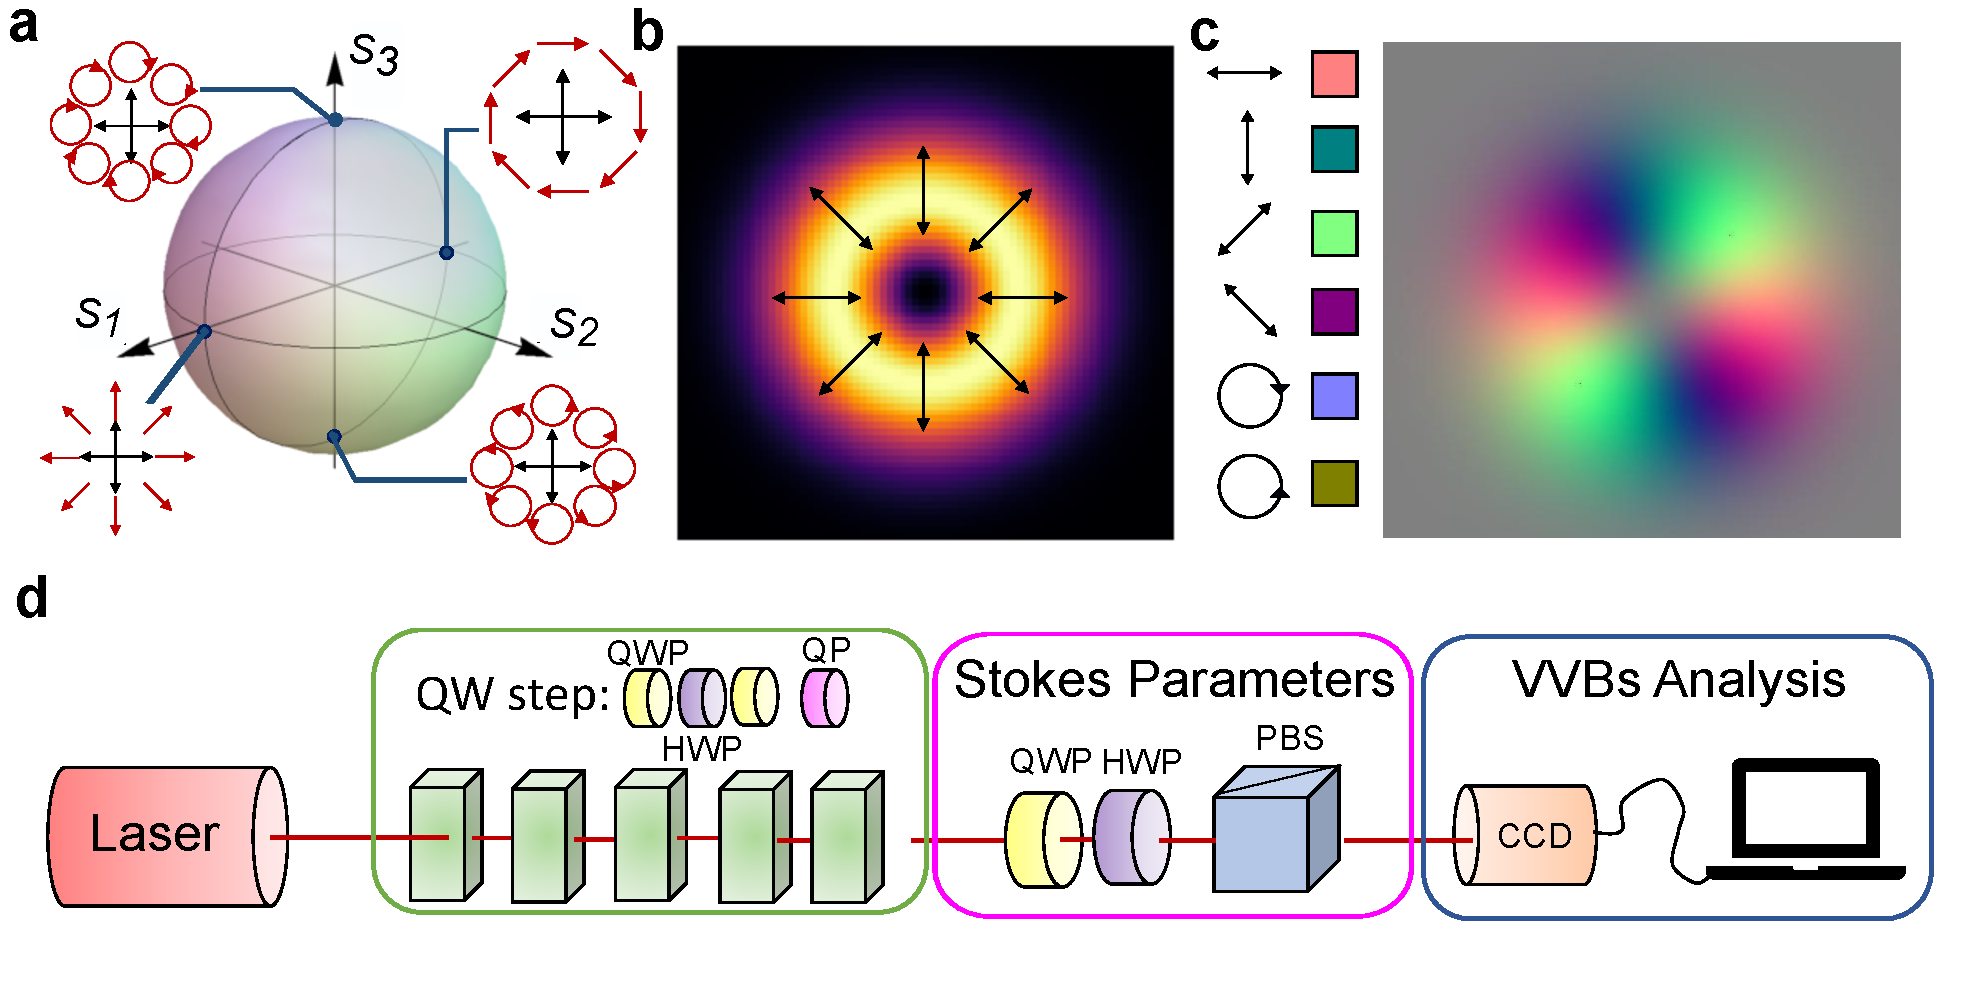
\includegraphics[width=0.8\textwidth]{VVBs-Fig1.pdf}
    \caption{
    	\textbf{(a)} High-order Poincar\'e sphere representation for $|m_{1,2}|=1$. Each point on the sphere corresponds to a VVB. 
	    \textbf{(b)} The intensity profile of a radially polarised \ac{VVB}, in which the polarisation direction always points outwards from the centre.
	    \textbf{(c)} An example of a colour-encoded VVB.
	    The legend reports the correspondence between colours and the different polarisations.
	    \textbf{(d)} Simple schematic of the experimental apparatus used to generate the \acp{VVB}. A continuous-wave laser emits a Gaussian beam $\on{TEM}_{00}$ at $\SI{808}{\nm}$. The light undergoes a $5$-step QW evolution, realised through a sequence of waveplates and QPs.
    	A CCD camera-based detection stage acquires the output intensity profiles, after projecting onto different polarisation states, thus allowing to compute the associated Stokes parameters.
    }%
    \label{fig:VVBs:poinc_sphere}
\end{figure}


\section{Experimental generation of Vector Vortex Beams}

\tmpHeading{VVBs}
\acfp{VVB} are superpositions of orthogonal polarisations states coupled with different \ac{OAM} states~\cite{padgett2004lights}.
More specifically, the electric field $\bs{E}_{m_1m_2p}$ of a \ac{VVB} decomposes as the sum of two~\ac{LG} modes with same $p$ and different azimuthal numbers $m_1>m_2$ carried by orthogonal polarisations:
\begin{equation}
	\bs{E}_{m_1m_2p} =
	\bs{e}_L \cos(\theta/2)\on{LG}_{m_1p} +
	\bs{e}_R e^{i \phi} \sin(\theta/2)\on{LG}_{m_2p},
	\label{eq:VVBs:definition_VVBs_field}
\end{equation}
where $\theta\in[0,\pi], \phi\in[0,2\pi]$ and the unit vectors $\bs{e}_{L,R}$ represent left and right circular polarisation, respectively.
For the purpose of this work we can ignore the radial number, fixing $p=0$.
For any given value of the parameters $(m_1, m_2, \theta, \phi)$, the polarisation pattern of a \ac{VVB} can be represented as a point in a \emph{generalised Poincar\'e sphere}, as also shown in~\cref{fig:VVBs:poinc_sphere}.
% In particular, we use the higher-order Poincar\'e representation in which the poles represent eigenstates of the total angular momentum but with opposite signs~\cite{milione2011higherorder}.
Each VVB can be characterised via its \emph{Stokes parameters} $(S_1,S_2,S_3)$.
These are defined in terms of the output intensities associated to different polarisation measurements.
Projecting the polarisation onto the three standard mutually unbiased bases, $b_1=(H,V), b_2=(D,A), b_3=(L,R)$, and denoting the two intensities corresponding to a given basis $b_j$ with $(I_{b_j,1},I_{b_j,2})$, the Stokes parameters are defined as
\begin{equation}
	S_{b_j} = \frac{I_{b_j,1}-I_{b_j,2}}{I_{b_j,1}+I_{b_j,2}}.
\end{equation}
%This is a way to characterise a state via its \emph{Stokes parameters} at every point of the transverse %profile.
%To do this, we first measure the output intensities $I_{b_j,1},I_{b_j,2}$ associated to a given choice of %polarisation basis $b_j$, and then compute the value of the corresponding Stokes parameter $S_{b_j}$ as %$S_{b_j}=(I_{b_j,1}-I_{b_j,2})/(I_{b_j,1}+I_{b_j,2})$.
%The canonical choice for the polarisation bases is $b_1=(H,V), b_2=(D,A)$ and $b_3=(L,R)$.
%%
It is worth noting that the Stokes parameters are the classical counterparts of the coordinates of density matrices in state space, upon replacement of intensities with probabilities.
In particular, for states living in a two-dimensional space, the Stokes parameters correspond to the coordinates in the Bloch sphere (which is often referred to as a \emph{Poincaré sphere} in this context).

\tmpHeading{Experimental generation and detection of VVBs}
As already discussed in~\cref{chapter:experimental_engineering_qudits}, we generate VVBs via polarisation-controlling waveplates interspersing $5$ cascaded QPs.
% This allows to generate VVBs with OAM quantum numbers taking odd values in the interval $\{-5,..,5\}$.
% Using different configurations of waveplates we can generate different VVBs.
% corresponding to different pairs $(m_1,m_2)$ of OAM quantum numbers, and parameters $(\theta, \phi)$.
The OAM azimuthal quantum numbers accessible with this scheme correspond to the walker states accessible via a $5$-step QW, that is, $\pm1,\pm3$, and $\pm5$.
Generated VVBs are characterised by the values of the three Stokes parameters at each point of their transverse profile. This amounts to collecting six intensities per pixel. The detection is carried out with a \ac{CCD} camera with resolution $1360 \times 1024$. 
We find, however, that a resolution of $128 \times 128$ is already sufficient for the tasks we consider, and the training stages are significantly sped up by reducing the resolution of the images (and thus the dimensionality of the handled data). We coarse-grain the images by integrating sub-matrices of the appropriate dimensions.

\tmpHeading{Colour-encoding VVBs}
To represent visually the polarisation patterns of VVBs, we use a Red-Green-Blue (RGB) colour encoding, mapping each $S_j$ into the strength of one of the primary colours.
More precisely, for each pixel of the CCD, the value of the red channel is set to $255\times(S_1+1)/2$, so that the red channel is saturated when $S_1=1$ and empty when $S_1=-1$ (remembering that $S_i\in[-1,1]$). Green and blue channels are defined similarly with $S_2$ and $S_3$.
An example of such colour encoding is given in~\cref{fig:VVBs:poinc_sphere}.
These images can also be understood as vectors of length $3\times M$ with $M$ the total number of pixels supported by the CCD camera. These vectors are what the ML algorithms use.

% \tmpHeading{Imperfections in the OAM beams generation}
% \Cref{eq_si:qplate} summarises the action of the QPs on LG modes.
% The output fields generated by such devices are \textit{Hypergeometric-Gaussian modes} (HyGG), an over-complete family of solutions to Helmholtz equation that display a phase term $e^{i m \phi}$ as the LG beams~\cite{Karimi:07}. Their expression in cylindrical coordinates $(r,\phi,z)$ is
% \begin{align}
%     \text{HyGG}_{p'm} & = i^{|m| +1} \sqrt{\frac{2^{p'+|m|+1}}{\pi \Gamma (p'+|m|+1)}}\frac{\Gamma(1+\frac{p'}{2}+|m|)}{\Gamma(|m|+1)} \notag\\
%     & \times \zeta^{\frac{p'}{2}}(\zeta + i)^{-(1+|m|+\frac{p'}{2})} \rho^{|m|} e^{\frac{-(i \rho^2)}{\zeta + i}} \notag \\
%     & \times {}_{1}F_1\left( -\frac{p'}{2}, 1 + |m|; \frac{\rho^2}{\zeta(\zeta+i)}\right) e^{i m \phi},
% \end{align}
% %
% where $\zeta={z}/{z_R}$ ($z_R$ is the Rayleigh range), $\rho ={r}/{w_0}$ with $w_0$ the beam waist, and ${}_{1}F_{1}$ the Hypergeometric function.
% \begin{figure}[tb]
%     \centering
%     \includegraphics[width=0.8\textwidth]{VVBs-hyGG.pdf}
%     \caption{
%     	\textbf{Role of the radial modes.}
%     	Simulated images of a VVB generated with HyGG modes. In the calculation we have considered two HyGG modes with $(m_1,m_2)=(-3,1)$ propagating for $z\sim 1\,m$ with a Rayleigh range $z_R\sim 4\,m$. Comparison of the intensities recorded in the polarization measurements in the experiment.
%     }
%     \label{fig:VVBs:hyGG}
% \end{figure}

% The transformation actually operated by a $q$-plate with $q=0.5$ on a LG modes with zero radial number is 
% \cite{Karimi:09}
% \begin{align}
%   \Vec{e}_L \text{ LG}_m &\stackrel{\text{QP}}{\longrightarrow} \Vec{e}_R\,\text{HyGG}_{|m|-|m+1|,m+1}   
% \end{align}
% The resulting HyGG beam carries OAM equal to $m+1$, but when expressed in the LG basis, it comprises the superposition of several modes with non-zero radial number, namely $\text{HyGG}_{|m|-|m+1|,m+1}=\sum_p c_p \text{LG}_{p,m+1}$. The contributions of the radial modes with $p>0$ can be neglected for $\zeta \ll 1$ and large $m$. For a detailed description of the coefficients $c_p$ see~\cite{Karimi:07,Karimi:09, cardano2015quantum}.

% In~\cref{fig:VVBs:hyGG} we report the comparison between the simulated images computed by considering HyGG modes instead of LGs and images recorded in the experiment. The two vortexes in the VVB carry respectively OAM equal to $(m_1,m_2)=(-3,1)$, more precisely we consider a state in the form $ \Vec{e}_R\,\text{HyGG}_{-1,-3}+\Vec{e}_L\,\text{HyGG}_{-1,1}$. The simulation's parameters, such as $\zeta$, were adapted to reproduce the conditions of the experiment.

% Even if such simple model of the experimental imperfections seems to be fit for the purpose, it is worth noting that other sources of noise could be investigated. First, in our simple model of the radial-mode contribution via HyGG modes, we did not consider the step-by-step conversion 
% operated by the cascaded $q$-plate system in the setup. A more rigorous calculation could take into account the propagation and conversion of the several radial contributions at each step. Other effects in this direction are the non ideal conversion efficiencies: residual lower-$m$ components propagate inside the principal beam and can modify the polarization pattern and the relative weights of the radial modes. In the end, relative misalignment among $q$-plates singularities could affects the quality of the VVBs.

% While the inclusion of all such considerations in the calculation of the training set could enhance the performance of a classifier in labelling experimental data, we leave it as a  perspective for a future work. On the other hand, a rigorous model of the imperfections is a complex task and makes the training set tied to the specifics of the experimental apparatus. Consequently, including some experimental images in the training set remains a possible solution.

% These were obtained with a CNN composed of three convolutional and max-pooling layers, and two fully connected layers. Each convolutional layer uses $32$ filters of size $3\times3\times3$, with ReLU activation function. The pooling layers apply the max operation to blocks of size $2\times2\times3$. Finally, the fully connected layers use the softmax activation function, defined as $\bs x\mapsto (e^{x_i}/\sum_j e^{x_j})_i$.

% \href{https://github.com/lucainnocenti/ML-classification-of-VVBs}{lucainnocenti/ML-classification-of-VVBs}.}

\begin{figure}[tb]
	\centering
	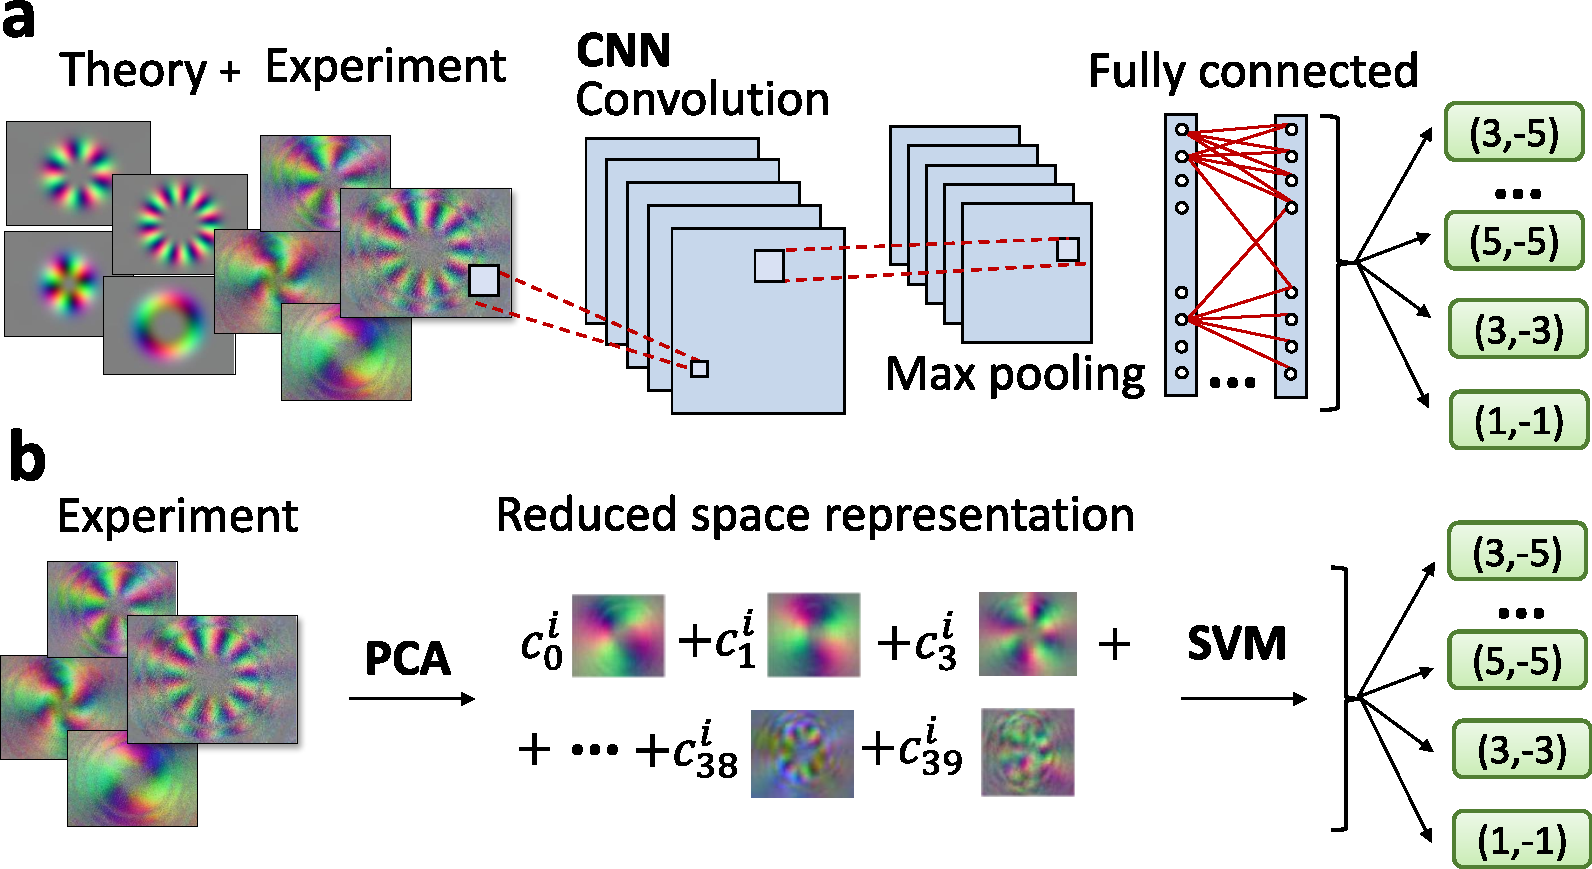
\includegraphics[width=0.82\textwidth]{VVBs-classification_pipelines_allgreen.pdf}
	\caption{
	Outline of classification scheme via CNNs \textbf{(a)} and PCA+SVM \textbf{(b)}.
	When using the CNN, the network is fed with complete images.
	On the other hand, the SVM classifier is fed with the reduced representation of the images, obtained via PCA.
	}
	\label{fig:VVBs:class_techniques}
\end{figure}


\section{Convolutional neural networks}
\label{sec:VVBs:CNNs}

\tmpHeading{What do we use CNNs for?}
We showcase the potential of \acp{CNN} to characterise experimentally generated states.
In particular, we test CNNs on two separate classification tasks:
1) finding the OAM numbers $(m_1,m_2)$ corresponding to input VVBs and 2) assuming a dataset of VVBs with fixed $(m_1,m_2)$, finding the values of $(\theta,\phi)$ characterising each VVB image.

\tmpHeading{What are CNNs?}
\acp{CNN} are translation-invariant deep NNs designed to handle image classification tasks~\cite{lecun2015deep}. Among their countless applications, CNNs have been used to recognise off-centre images and segmented handwritten digits~\cite{simard2003best,ciresan2011flexible},
and for facial recognition tasks~\cite{matsugu2003subject}.
In its simplest form, a \ac{CNN} consists of a \emph{convolutional layer},
 % which consists of a series of nonlinear transformations applied to the input images,
followed by a \emph{max-pooling layer}, and finally a \emph{fully connected layer}, as also shown schematically in~\cref{fig:VVBs:class_techniques}.
These build up a mapping from each image to one of a finite number of output \emph{classes} defining the problem under consideration. In our case, the classes would be the $(m_1,m_2)$ pairs.
More precisely, the different layers operate as follows:
\begin{itemize}
	\item (\textbf{\emph{Convolutional layer}})
		The idea of the convolutional layer is to extract local features from the image.
		This is done by computing the inner product of every $k\times k$ block of the image with a fixed $k\times k$ matrix, referred to as a \emph{filter} in this context. The filter is applied sequentially to each $k\times k$ block of the image. This is also shown schematically in~\cref{fig:VVBs:convolutions_example}.
		% The size of these steps is known as the \emph{stride}. A stride of $1$ corresponds to the filter being applied to every single $k\times k$ contiguous block of the input.
		% Larger strides mean that some blocks are skipped.
		Each such filter extracts a specific feature from the image. The output of this process is called a \emph{feature map}. Multiple filters, and thus multiple feature maps, can be applied to the same image, to extract different features.
		% The values of the filters, as well as the weights and biases of their connections with their input, are parameters to be trained.
		If the input images have dimensions $n_{ch}\times N_x\times N_y$, with $N_x,N_y$ width and height and $n_{ch}$ the number of \emph{channels} of the image (\emph{e.g.} $n_{ch}=3$ for RGB images), then a convolutional layer with $N_c$ filters will produce an output of size $N_c\times N_x\times N_y$.
		Convolutional layers are typically followed by a nonlinear function, applied elementwise to the outputs. A common choice is the so-called Rectified Linear Unit (ReLU), defined as $x\mapsto\max(x,0)$.
		Introducing nonlinearity is crucial, lest the whole process be linear and thus unable to capture interesting features.
		Explicitly, we write each input image as a three-index tensor $\calI_{\alpha,ij}\equiv\calI^\alpha_{ij}$, with $\alpha=1,2,3$ the colour channels and $i,j=1,...,128$ indexing the pixels.
		Writing the filters as a tensor $\calF_{k\alpha mn}\equiv\calF^{k\alpha}_{mn}$, with $k=1,..,32$ indexing the different filters, we can compute the activation maps $\calM_{k\alpha pq}$ as
		\begin{equation}
			\calM_{k\alpha pq} = (\calF^{k\alpha}\star\calI^{\alpha})_{pq} \equiv
			\sum_{mn} \calF^{k\alpha}_{mn} \calI^\alpha_{R[p,q]_{mn}},
		\end{equation}
		where $\star$ denotes the $2$D convolution operation, which consists in computing the inner product of $\calF^{k\alpha}$ with the different $3\times3$ blocks of $\calI^\alpha$. Here, $R[p,q]$ denotes the indices of a $3\times3$ block surrounding the indices $p,q$.
		Explicitly, $R[p,q]_{mn}\equiv (p+m-2,q+n-2)$ with $m,n=1,2,3$, so that for example $R[1,1]$ covers the $3\times3$ submatrix surrounding the $(1,1)$ element of the image (which is the upper-left pixel). Whenever $R[p,q]$ covers pixels that fall outside of the boundaries of the image, like is the case for $R[1,1]$, it is standard practice to apply some \emph{padding} to the image, which in this case amounts to adding a single row or column of zeros on each side of the image. This is done to avoid having the bordering pixels being given a lesser weight than the rest.
		Once the activation maps are computed, the ReLU activation function is applied element-wise to $\calM_{k\alpha pq}$.
	\item (\textbf{\emph{Pooling layer}})
		After convolution and nonlinearity follows a \emph{max-pooling} stage. Here, the feature maps are down-sampled, by partitioning each feature map into blocks of size $\ell\times \ell$, and mapping each such block into its maximum value (other types of pooling are possible, for example by mapping each block into its average value).
		This is used to retain only the most relevant features from the feature maps, thus reducing noise and increasing the efficiency of training.
	\item (\textbf{\emph{Fully connected layer}})
		A fully connected layer is finally applied to the output of the max-pooling stage.
		This stage operates like a standard NN layer.
		This is the layer in which the networks takes a decision as to which class the input image belongs to: the chosen class is the one corresponding to the output neuron with the largest activation.
		More precisely, such a fully connected NN takes as input an array $\bs x^{\on{in}}$ and applies an affine transformation, effectively implementing the mapping
		\begin{equation}
			\bs x^{\on{in}}\mapsto \bs x^{\on{out}}
			\equiv
			\left(
				\sum_k w_{jk} x^{\on{in}}_k + b_j
			\right)_j,
		\end{equation}
		where $\bs x^{\on{out}}$ is a vector of length equal to the number of output neurons (in the cases studied here, the number of output classes), and the parameters $w_{jk},b_j$ are referred to as the \emph{weights} and \emph{biases} of the network. The output of the network is obtained by applying a nonlinear function, often the \emph{sigmoid function} $\sigma(x)\equiv 1/(1+e^{-x})$, to the outputs.
		In the context of our CNN, this fully connected layer takes as input the set of outputs of the previous max-pooling layer (simple flattening is applied to convert the three-dimensional tensors produced by the pooling layers into a form suitable for the fully connected layer).
\end{itemize}
Note that this is only the most basic structure found in CNNs. Actual CNNs will often contain different numbers of convolutional, pooling, and fully connected layers in different arrangements and with different parameters, depending on the specific applications.

\tmpHeading{Training the network}
The free parameters of the CNN, which comprise the weights and biases connecting the neurons at different layers, as well as the values of the filters, are trained using \ac{SGD}. This is the same algorithm described in~\cref{subsec:GL:supervised_learning_and_SGD}.
\ac{SGD} operates by first initialising the parameters with random values, then using a \emph{batch} of training images $\{(\bs x_k,\ell_k)\}_k$ to compute the Euclidean distance between the outputs produced by the network when fed with the images, and the corresponding labels (which are the outputs the network should give when ideally trained).
Here, $\bs x_k$ denote the input images, while $\ell_k$ the class corresponding to the $k$-th image, expressed as an integer number.
This distance is used as the \emph{cost function} that the algorithm seeks to minimise.
Denoting with $f_\bslambda$ the mapping implemented by the network when its parameters have values $\bslambda$, this distance reads
\begin{equation}
	L_\bslambda(\bs x_k,\ell_k) = \frac{1}{N_{\on{batch}}}
	\sum_k \|f_\bslambda(\bs x_k)-\bs e_{\ell_k}\|^2,
\end{equation}
where $N_{\on{batch}}$ is the number of elements in the batch, and $\bs e_{\ell_k}$ is the vector with size equal to the number of classes, and elements $(\bs e_{\ell_k})_j=\delta_{j,\ell_k}$.
We then tune the parameters of the network to make this distance smaller, by updating them in the direction of the gradient of the distance function:
\begin{equation}
	\bslambda \to
	\bslambda - \eta \nabla_\bslambda f_\bslambda(\bs x_k),
	\label{eq:VVBs:naive_updating_rule}
\end{equation}
where the real parameter $\eta>0$ is the \emph{learning rate}, which determines the speed of the training.
In actual implementation, we often use variations of~\cref{eq:VVBs:naive_updating_rule} that are more robust and converge quicker in most applications.
An updating rule that is often used in state-of-the-art applications is the so-called \textsc{Adam} optimiser~\cite{ruder2016overview}, which uses different learning rates for different parameters, and adapts it conditionally to the recent training history of that parameter.
To build and train the \acp{CNN} we use the Python library \emph{Keras}~\cite{chollet2015keras}.

% channel1 = ConstantArray[0, {7, 7}];
% channel1[[2 ;; 6, 2 ;; 6]] = RandomInteger[{0, 2}, {5, 5}];
% channel2 = ConstantArray[0, {7, 7}];
% channel2[[2 ;; 6, 2 ;; 6]] = RandomInteger[{0, 2}, {5, 5}];
% channel3 = ConstantArray[0, {7, 7}];
% channel3[[2 ;; 6, 2 ;; 6]] = RandomInteger[{0, 2}, {5, 5}];

% filter1 = RandomInteger[{-1, 1}, {3, 3}];
% filter2 = RandomInteger[{-1, 1}, {3, 3}];
% filter3 = RandomInteger[{-1, 1}, {3, 3}];

% grayBorderingSquares[size_Integer] := {LightGray,
%      Rectangle[{#1, #2} - 0.45, {#1, #2} + 0.45] &[##]
%      } & @@@ Select[
%     Tuples[Range@size, {2}],
%     Min@# == 1 || Max@# == size &
%     ];
% greenInsideSquares[size_Integer] := {LightGreen,
%      Rectangle[{#1, #2} - 0.45, {#1, #2} + 0.45] &[##]
%      } & @@@ Select[
%     Tuples[Range@7, {2}],
%     Min@# > 1 && Max@# < size &
%     ];
% squaresGrid[xs_, ys_, color_] := {color,
%    Rectangle[{#[[1]], #[[2]]} - 0.45, {#[[1]], #[[2]]} + 0.45] & /@ 
%     Tuples@{xs, ys}
%    };

% numbersInMatrix[matrix_] := Table[
%    Text[matrix[[Dimensions[matrix][[2]] + 1 - j, i]], {i, j}],
%    {i, 1, Dimensions[matrix][[1]]}, {j, 1, Dimensions[matrix][[2]]}
%    ];

% tripleCopy[expr_, size_] := 
%   Translate[expr, {0, #}] & /@ {0, -size - 1, -2 size - 2};

% fig = With[{size = Length@channel1}, Graphics[{
%     {grayBorderingSquares@size, greenInsideSquares@size} // 
%      tripleCopy[#, size] &,
%     Translate[numbersInMatrix@#[[1]], {0, #[[2]]}] & /@ Thread@{
%        {channel1, channel2, channel3}, {0, -size - 1, -2 size - 2}
%        }
%     (*{FaceForm[],EdgeForm[{Thick,Red}],Rectangle[{#2,
%     size+1-#1}-0.45,{#2,size+1-#1}+0.45]&[1,3]}*)
%     , 
%     tripleCopy[#, size] &@
%      {FaceForm[], EdgeForm[{Thickness@0.01, Red}], 
%       Rectangle[{5, 5} - 0.48, {7, 7} + 0.45] &[1, 3]},
%     Sequence @@ With[{xmin = 7, xmax = 12.5},
%       tripleCopy[#, size] &@
%        {Thick, Dashed, Red,
%         {Line@{{xmin, 4.5}, {xmax, 4.5}}},
%         {Line@{{xmin, 7.5}, {xmax, 7.5}}},
%         {Line@{{xmax - 3, 4.5}, {xmax - 3, 7.5}}},
%         {Line@{{xmax, 4.5}, {xmax, 7.5}}}}
%       ],
%     squaresGrid[Range[10, 12], Range[5, 7], LightRed] // 
%      tripleCopy[#, size] &,
%     Translate[numbersInMatrix[filter1], {9, 4}],
%     Translate[numbersInMatrix[filter2], {9, 4 - size - 1}],
%     Translate[numbersInMatrix[filter3], {9, 4 - 2 size - 2}],
%     Arrow@{{13, 6}, {15, 6}} // tripleCopy[#, size] &,
%     {FaceForm[], EdgeForm[{Black, Thick, Dashed}], 
%       Rectangle[{16, 6} - 0.5, {16, 6} + 0.5]} // 
%      tripleCopy[#, size] &,
%     Text[Style[
%       Total[Flatten@channel1[[;; 3, 5 ;; 7]]*Flatten@filter1], 
%       Bold], {16, 6}],
%     Text[Style[
%       Total[Flatten@channel2[[;; 3, 5 ;; 7]]*Flatten@filter2], 
%       Bold], {16, 6 - size - 1}],
%     Text[Style[
%       Total[Flatten@channel3[[;; 3, 5 ;; 7]]*Flatten@filter3], 
%       Bold], {16, 6 - 2 size - 2}]
%     }, ImageSize -> 300]]

\begin{figure}[tb]
    \centering
    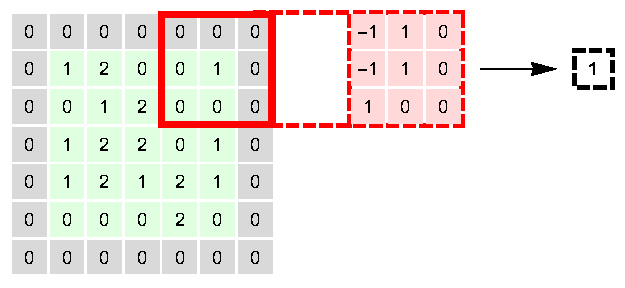
\includegraphics[width=0.5\linewidth]{VVBs-CNNconvolutions-scheme-1row}
    \caption{
    	Simple illustration of how a filter is applied to an input image.
    	The green square represents an input image, focussing on a single channel. In our notation, assuming the first channel, this would be $(\calI^1_{ij})_{ij}$ with $i,j=1,...,5$.
    	The gray squares represent the padding applied to the image.
    	The dashed red square is a $3\times 3$ filter, which is here shown applied to the upper-right $3\times3$ block of the image.
    	In our notation, the filter is $\calF^{1,1}$ (assuming $k=1$ for the first filter). The thick red square is $R[1,5]$. The dashed black rectangle on the right contains the result of computing the inner product of the filter with the highlighted block of the image.
    	Being the result $1>0$, the ReLU nonlinearity leaves it unchanged.
    }%
    \label{fig:VVBs:convolutions_example}
\end{figure}

\begin{figure}[t]
    \centering
    \includegraphics[width=0.7\textwidth]{VVBs-classification_with_CNN_schematics.pdf}
    \caption{
    	Comparison between simulated and experimental polarisation patterns for a sample of \acp{VVB}. Each image is produced by a VVB with OAM numbers $(m_1, m_2)$ belonging to one of the classes listed in the table.
    }%
    \label{fig:VVBs:simVsExp}
\end{figure}

\tmpHeading{Categorisation into discrete classes}
We first showcase CNNs to classify experimental and simulated VVBs into $15$ different classes characterised by their OAM numbers as per~\cref{fig:VVBs:simVsExp}.
For each class we consider states with $\theta=\pi/2$ and $\phi\in[0,2\pi]$.
We tested different CNN architectures, the details of which can be found in the \href{https://github.com/lucainnocenti/ML-classification-of-VVBs}{GitHub repository}~\footnote{https://github.com/lucainnocenti/ML-classification-of-VVBs}.
% The size of the training set is $400$ images per class.
\begin{itemize}
	\item Training and testing CNNs with simulated images leads to $100\%$ accuracy. This remains true when training and testing datasets comprise simulated images with added white noise.
	We achieved this already with a CNN using two convolutional layers, each using $16$ activation maps (that is, there are $16$ different filters used per convolutional layer), each followed by a max-pooling layer, and a final hidden fully connected layer with $32$ neurons, amounting to a total number of $\sim5$k trainable parameters.
	\item On the other hand, training on simulated images is not enough to teach the network to categorise experimental ones.
	We can improve the accuracy by applying \emph{pre-processing} to the training images. This consists of applying random transformation to artificially inflate the number of images available for training. Such transformations include random translation, rescalings, shearings and changes in overall brightness. A heavy use of pre-processing significantly improves performances, by tailoring the network to only pick up the features of the images which are relevant for the classification.
	A sample of the pre-processed images actually used in training is given in~\cref{fig:VVBs:pre-processed_images}.
	However, pre-processing does not push accuracies above $\sim60\%$.
	% We found that applying heavy pre-processing to the training images, that is, artificially inflating the images used for training by applying random transformation 
	A possible reason for this is that experimental images can be quite different from simulated ones. Indeed, simulated images assume a perfect superposition of two different OAM numbers, whereas the states produced by \acp{QP} are closer to \emph{Hypergeometric-Gaussian modes}~\cite{karimi2007hypergeometricgaussian}. These are an alternative family of solutions of the Helmoltz equation in cylindrical coordinates, which also display the $e^{im\phi}$ phase term, but model more closely the states produced by \acp{QP}.
	% We show examples of such beams in~\cref{fig:VVBs:hyGG}.
	In this work we stick with the simpler OAM beams for simplicity, but it is possible that using a better model for the simulation would allow to classify experimental images training solely on simulated ones.
	\item Finally, we find that a small number of experimental images are enough to allow the network to generalise and be able to categorise the rest of them.
	We train a CNN using $20$ experimental images per class, and test it on the remaining $\sim1700$ ones, and achieve a $\sim 99\%$ accuracy on the test set.
	We achieve this using a CNN using three convolutional layers followed by a max-pooling layer each, and a hidden fully connected layer with $64$ neurons, amounting to a total of $\sim38$k parameters. The history of accuracies per epoch for training and validation sets is reported in~\cref{fig:VVBs:training_history}.
\end{itemize}

% \begin{figure}[tb]
%     \centering
%     \includegraphics[width=0.7\linewidth]{Figures/VVBs/VVBs-hyGG.pdf}
%     \caption{
%     	Comparison between simulated images of VVBs generated with HyGG modes. In the calculation we have considered two HyGG modes with $(m_1,m_2)=(-3,1)$ propagating for $z\sim 1\,m$ with a Rayleigh range $z_R\sim 4\,m$. Comparison of the intensities recorded in the polarization measurements in the experiment.
%     }%
%     \label{fig:VVBs:hyGG}
% \end{figure}

\begin{figure}[tb]
	\centering
	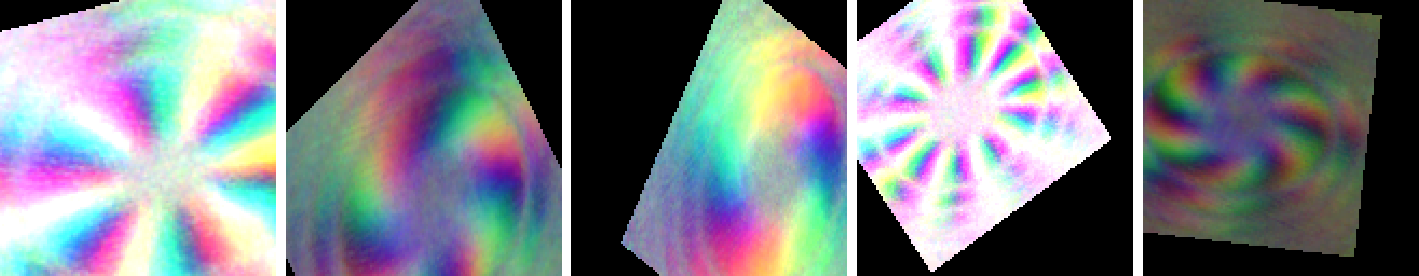
\includegraphics[width=\linewidth]{VVBs-training_examples.png}
	\caption{Sample of pre-processed training images used to train the CNN. These are obtained taking images of VVBs and applying random transformations such as translations, shearings, rescalings, changes in overall brightness. We also add random white noise to the images.
	This allows to substantially enlarge the size of the training dataset, while at the same time forcing the CNN to not pick up features --- such as the centering of the image or its overall brightness --- which we know should not be used to classify the images.
	}
	\label{fig:VVBs:pre-processed_images}
\end{figure}

\begin{figure}[t]
	\centering
	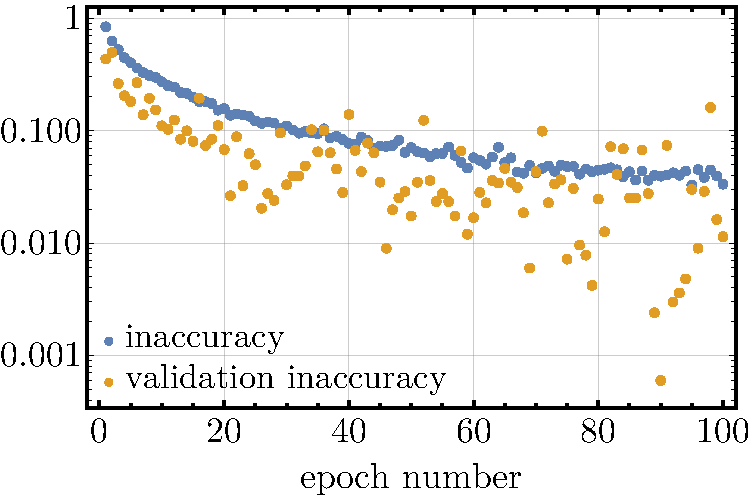
\includegraphics[width=0.6\linewidth]{VVBs-inaccuracy_training-history.pdf}
	\caption{History of training inaccuracy (here, $\on{inaccuracy}\equiv1-\on{accuracy}$) during training of the experimental VVBs. We give the inaccuracies computed over training and validation datasets for each training epoch. Each training epoch is composed of $200$ training steps, and in each step the network is trained on $32$ images.}
	\label{fig:VVBs:training_history}
\end{figure}

\tmpHeading{Retrieving the position in the Poincaré sphere}
We also test the network on a different problem: assuming $(m_1,m_2)$ is fixed, retrieve the parameters $(\theta,\phi)$ characterising the VVB (remembering the definition of VVBs as given in~\cref{eq:VVBs:definition_VVBs_field}).
In particular, we train a CNN to retrieve the values $(\theta,\phi)$ characterising VVBs corresponding to the OAM quantum numbers $m_1=-m_2=1$.
The network is thus trained to discriminate both rotations in the polarisation patterns (corresponding to changes of $\phi$), and variations in the colour tone (corresponding to changes of $\theta$).
To frame this as a classification task, we partition the sphere in $26$ disjoint sectors.
Working in spherical coordinates, we partition $\theta$ is in the $3$ intervals $\left[k \frac{\pi}{8}, (k+2) \frac{\pi}{8}\right]$ with $k=1,3,5$, and $\phi$ in the $8$ intervals $\left[t \frac{\pi}{4}, (t+1) \frac{\pi}{4}\right]$ with $t \in \{0,...,7\}$.
This leaves two classes surrounding the two poles of the sphere, corresponding to $\theta \in \left[0, \frac{\pi}{8}\right]$ and $\theta\in\left[ \frac{7}{8} \pi, \pi\right]$.
Partitioning makes the classification of VVBs closer to the border of two sectors harder, but nonetheless provides useful information about the suitability of CNNs for this kind of task.
We train the CNN with $500$ simulated images per class in the training set, and $125$ per class in the validation one. The maximum accuracy  achieved is $\sim 0.90$.
The suboptimality of this result can be understood as consequence of framing the problem as a classification task. Training a CNN for the corresponding regression task will potentially give much better results. This is however generally a nontrivial task. We will thus here choose a different route to approach this regression task, leveraging dimensionality reduction paired with SVM classifiers, as discussed in the next sections.


\section{Dimensionality reduction}
\label{sec:VVBs:dimensionality_reduction}

\tmpHeading{A different approach to classify images}
While CNNs provide good performance for general image classification tasks, the specific structure of the datasets we deal with can be leveraged to make for more efficient algorithms. In particular, we know that the datasets consist of intensity patterns associated with (mostly pure) quantum states.
% we can hope to achieve similar performances in the tasks we are interested in by exploiting additional structure that we know is intrinsic to our dataset, due to it consisting of a set of intensities associated with states of light.
In this section we present alternative approaches to extract information the dataset of interest, using \ac{DR} to expose the intrinsic structure of the dataset.


\tmpHeading{DR and PCA}
\acf{DR} is a class of algorithms whose goal is to find low-dimensional encodings of high-dimensional datasets~\cite{cunningham2008dimension,fodor2002survey}.
This has several applications, from data visualisation, to improving the efficiency of classification and regression algorithms, which can be applied on the reduced representation of the data.
A classical \ac{DR} algorithm is \acf{PCA}.
In its simplest form, \ac{PCA} is a \emph{linear} \ac{DR} algorithm which, given a dataset of vectors in a high-dimensional space $\RR^n$, finds the directions which capture the maximum amount of information about the dataset~\cite{jolliffe2011principal,jolliffe2016principal}.
More specifically, given a dataset comprised of $N$ real vectors of length $M$, we define the \emph{data matrix} $\bs X$ as the $N\times M$ matrix whose $i$-th row is the $i$-th dataset vector. \ac{PCA} then finds the vectors $\bs a\in\RR^{M}$ that maximise the variance of $\bs X\bs a$. This turns out to be equivalent to diagonalising $\bs S\equiv \tilde{\bs X}^T\tilde{\bs X}/(N-1)$, where $\tilde{\bs X}$ is the \emph{centered data matrix}, which is equal to $\bs X$ modulo each of its columns shifted in order to average to zero.
The first $k$ \emph{principal components} found by \ac{PCA} are then the $k$ eigenvectors of $\bs S$ corresponding to the largest $k$ eigenvalues.
Note that these principal components are themselves vectors of the same ``type'' as the data vectors. This means that \ac{PCA} effectively generates a set of data vectors which ``optimally represent'' the information content of the given dataset.

\tmpHeading{PCA and VVBs}
The rationale behind using \ac{PCA} in the context of \acp{VVB} is that, although experimental images live in extremely high-dimensional spaces (whose dimension is of the order of the number of pixels of the \ac{CCD} camera), the underlying dimension of the generated \acp{VVB} is typically much lower.
This means that, although the experimental dataset might \emph{a priori} seem like a complicated bundle of high-dimensional vectors, the underlying data is actually characterizable by a small number of parameters.
% Furthermore, the linearity of the mapping from the full to the reduced space makes it preserve many of its geometrical properties.
This is a form of \emph{unsupervised} learning, in that we gain useful information about the the images without feeding the algorithm with any prior knowledge about their structure.


% \tmpHeading{For example...}
% For example, in our case, each row of $\bs X$ is a vector of length $128\times128\times3$ containing the Stokes parameters $S_{b_1}, S_{b_2}, S_{b_3}$ for each pixel of the camera.
% Because each image corresponds to such a vector, and vice versa each such vector corresponds to the image of a \ac{VVB}, we can represent the principal components found by \ac{PCA} again in the form of images, which allows us to gain some intuition into the type of principal components that optimally represent the data according to \ac{PCA}.


\subsection{Retrieving states from probabilities}

\tmpHeading{Measuring in a single measurement basis}
Collecting experimental intensity images with the \ac{CCD} camera is akin to measuring output probabilities in a fixed measurement basis.
In general, this is not sufficient to fully reconstruct a state.
However, specific conditions (such as sparsity of the state and an appropriate choice of measurement basis) still allow for a full reconstruction~\cite{banchi2018multiphoton}.
More specifically, let $\rho$ be the density matrix characterising a state, and let us assume that this state is low-rank (that is, only a small number $n$ of eigenvalues of $\rho$ are non-vanishing).
The output probabilities in the computational basis following evolution through a unitary $\calU$ are
\begin{equation}
	p_k = (\calU\rho\calU^\dagger)_{kk}
	    = \sum_{ij}\calU_{ki}\bar\calU_{kj}\rho_{ij}.
\end{equation}
% Note that this situation models what happens when we measure VVBs with a CCD camera: VVBs are sparse in the OAM-polarisation basis (they are effectively two-dimensional), and measurement in the position basis can be described as a projective measurement following a unitary $\calU$ describing the change of basis.
The mapping between density matrices and detected probabilities is thus $\bs p=\Psi(\rho)$ where $\Psi$ is the linear operator
$\Psi\equiv\sum_j \ketbra{j}{jj}(\calU\otimes\calU^*)$.
This operator can equivalently be represented as a matrix with elements
$\Psi_{i,jk} = \calU_{ij}\calU^*_{ik}$.
Equivalently, we can represent $\rho$ in a basis of Hermitian operators as $\rho=\sum_k c_k \sigma_k$. We then have the induced linear mapping $p_j = \sum_k \tilde\Psi_{jk}c_k$, with $\tilde\Psi_{jk}\equiv\Psi(\sigma_k)_j$.
This linearity implies that many geometrical features of the space of states are preserved in the space of probabilities. Moreover, a suitable choice of $\Psi$ will allow to retrieve $\rho$ from the knowledge of $\bs p$.
For this to be possible, $\Psi$ needs to have a number of rows greater than or equal to the number of columns. Physically, this amounts to the measurement basis containing a sufficient number of elements. More specifically, $\Psi$ needs to be \emph{left-invertible}, which is the case when its columns are linearly independent.

\tmpHeading{Application to experimental VVB images}
In our case, $\rho$ is a description of a VVB in the OAM-polarisation basis, which is the basis in which it is sparse, while $\calU$ is the unitary mapping this basis into the position basis, which is the one that CCD cameras naturally operate on. In principle, one might need to take care of the different dimensionality of these spaces (the OAM space is countable while the position one is not), but this is easily fixed by discretising the position space, which is what is done naturally by the finite number of pixels of the CCD camera. 
The set of detected probabilities is then given by $\bs p=\on{diag}(\calU\rho\calU^\dagger)\equiv\Psi(\rho)$.
Crucially, the linearity of $\Psi$ implies that it preserves the \emph{convexity} of the space of states.
For example, if we consider the set of states of the form $c_0 \ket{\uparrow,m=m_1} + c_1 \ket{\downarrow,m=m_2}$ with $m_1\neq m_2$, the corresponding density matrices will be arranged to form a three-dimensional sphere embedded in the full state space (because these are effectively different states of a single qubit).
Thanks to the linearity of $\Psi$, \emph{the corresponding probabilities $\bs p$ will also be contained in a spherical surface}, up to possible rescaling of the axes.
In other words, the Bloch sphere of the original two-dimensional system is still present, albeit hidden, in the experimental images, embedded into an extremely high-dimensional space.


\begin{figure}[tb]
    \centering
    \includegraphics[width=0.8\linewidth]{VVBs-Fig4.pdf}
    \caption{
		\textbf{(a)}
		High order Poincaré sphere for \acp{VVB} with $|m_{1,2}|=1$. Magenta-coloured parallels (Blue-coloured meridians) mark intervals between consecutive values of $\theta$ ($\phi$). 
		Along a meridian the colours of the pattern vary from the hottest to the coldest one. Along a parallel, the patterns rotate.
		\textbf{(b)}
		Comparison between experimental and simulated \ac{VVB} images for different angles $(\theta, \phi)$.
		\textbf{(c)}
		Distribution of fidelities obtained comparing each experimental VVBs with its reduced 3D representations given by PCA. Projecting each image onto its first three principal axes and rescaling brings the data (orange points) onto a sphere in 3D, as shown in the inset. The inner (outer) black (semi-transparent) sphere is added for contrast [radius equal to that of the point with smaller (larger) radius].
		\textbf{(d)}
		Average prediction accuracy of a linear \ac{SVM} classifier, trained and tested after applying linear DR to the data, against the number of reduced dimensions $n_c$.
		For each of the 15 classes (cf.~\cref{fig:VVBs:simVsExp}) in which the experimental dataset was divided, we show in the inset the true-table. 
    }%
    \label{fig:VVBs:PCAresults}
\end{figure}


\subsection{Results}

\tmpHeading{PCA applied to experimental data}
As a notable example, we apply these observations to VVBs with $m_2=-m_1=1$.
These are the states of the form $c_0 \ket{L,m=1} + c_1 \ket{R, m=-1}$ with $\abs{c_0}^2+|c_1|^2=1$.
We find that applying PCA to a dataset of images corresponding to these VVBs naturally produces the underlying Bloch sphere representation:
the first three singular values are sufficient to capture most of the information, and projecting the images along the corresponding axes, the dataset is in good approximation arranged on a three-dimensional sphere.
Note that this is not straightforwardly deduced from the experimental images alone, but is easily found via \ac{DR}.
This result highlights the potential of \ac{DR} to reveal features of the states generating a given experimental dataset, also in the presence of experimental noisy conditions.
To assess the accuracy of such reconstruction, we compute the average fidelity $\calF_{\on{avg}}$ between the expected state and the one found by our analysis with PCA.
This is found to be $\calF_{\on{avg}}\sim0.96$, with standard deviation $\sim0.01$, thus certifying the quality of the reconstruction.
The full histogram of fidelities is given in~\cref{fig:VVBs:PCAresults}\textbf{c}, 

\begin{figure}[tb]
  \centering
  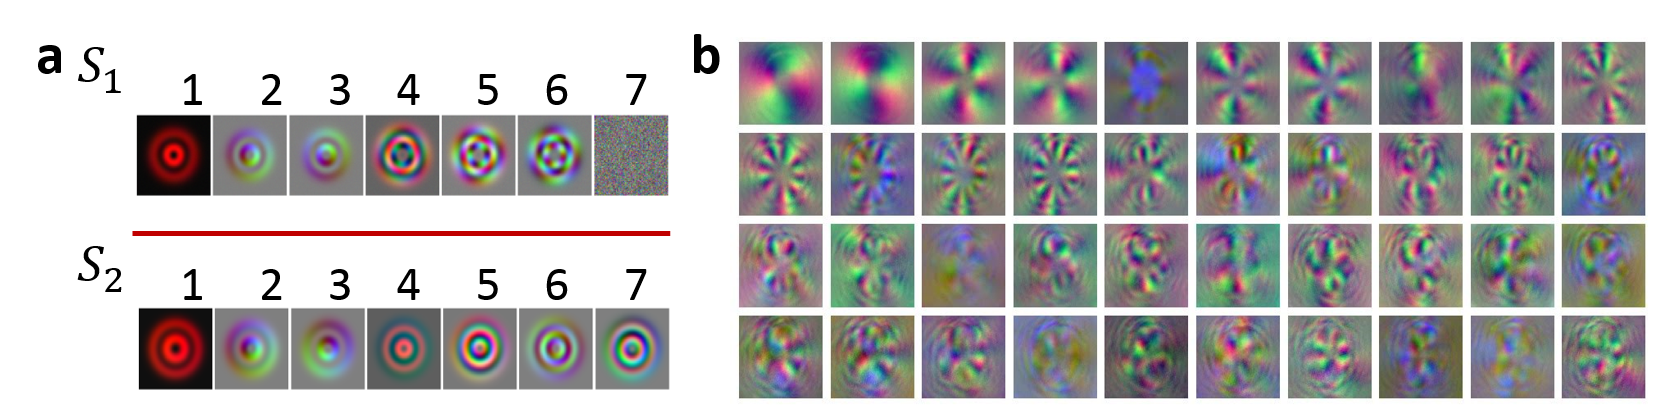
\includegraphics[width=0.98\textwidth]{S1_fig.png}
  \caption{
      \textbf{(a)}
       Principal components obtained using PCA on simulated datasets of noisy VVB. The first (second) row shows the first seven principal components obtained on the dataset $\mathcal S_1$ ($\mathcal S_2$). 
       The first 6 (all 7) components correspond to non-vanishing singular values.
       \textbf{(b)} First 40 principal components individuated in the experimental dataset corresponding to the 15 classes labelled by $(m_1,m_2)$, discussed in the main text.%
    }
    \label{fig:VVBs:principal_components}
\end{figure}

% \begin{figure}[tb]
%     \centering
%     \begin{minipage}{0.49\textwidth}
%         \centering
%         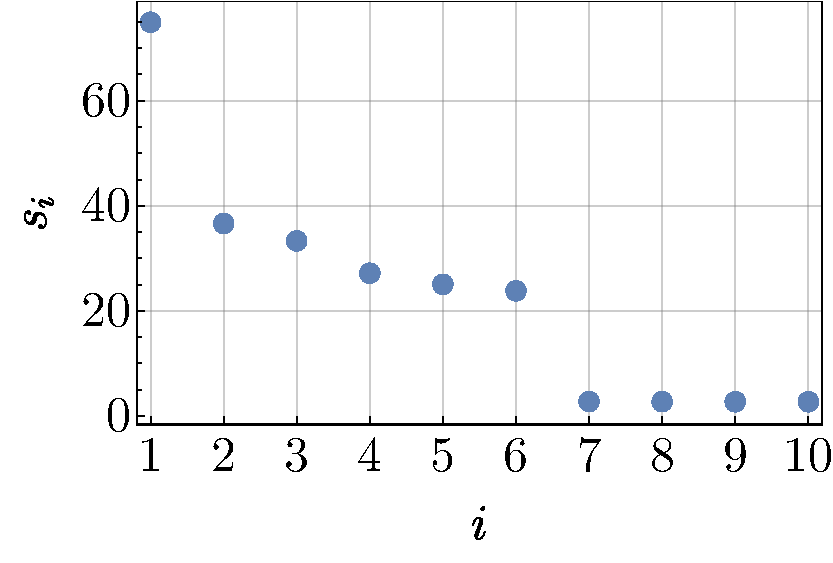
\includegraphics[width=0.99\textwidth]{VVBs-principalValues_sixNonzero.pdf} % first figure itself
%         \caption{first figure}
%     \end{minipage}\hfill
%     \begin{minipage}{0.49\textwidth}
%         \centering
%         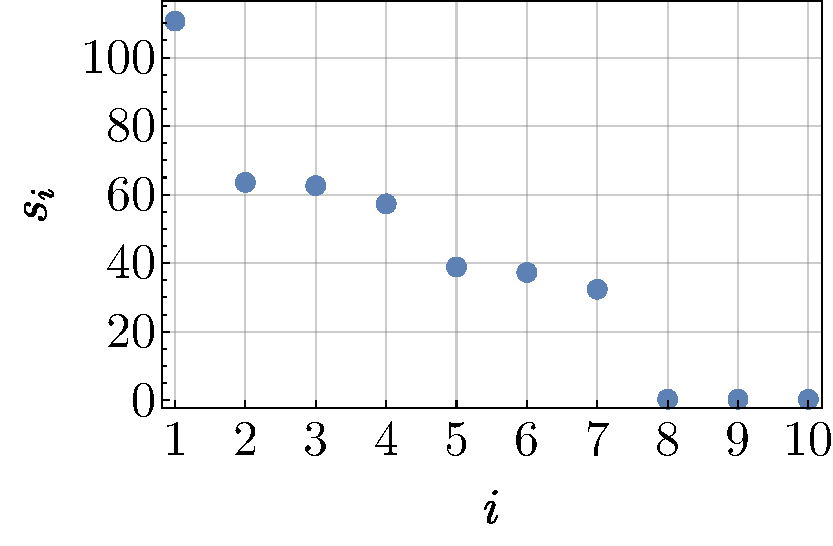
\includegraphics[width=0.99\textwidth]{VVBs-principalValues_sevenNonzero.pdf} % second figure itself
%         \caption{second figure}
%     \end{minipage}
% \end{figure}
\begin{figure}[tb]
    % \vspace{-50pt}
    \begin{subfigure}{0.5\textwidth}
        \centering
        \caption{}
        \label{fig:GL:toffoli_diagonal_solutions}
        \hspace{-20pt}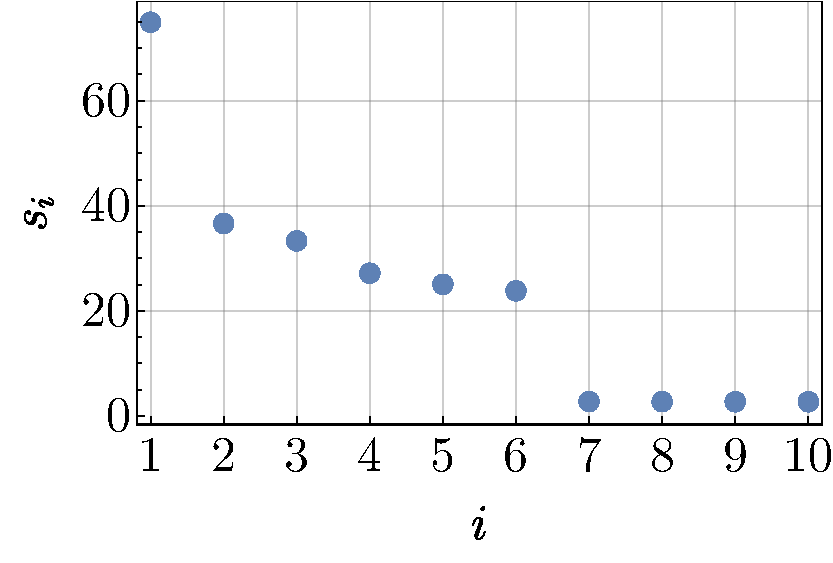
\includegraphics[width=\textwidth]{VVBs-principalValues_sixNonzero.pdf}
    \end{subfigure}%
    \begin{subfigure}{0.5\textwidth}
        \centering
        \caption{}
        \label{fig:GL:fredkin_diagonal_solutions}
        \hspace{-20pt}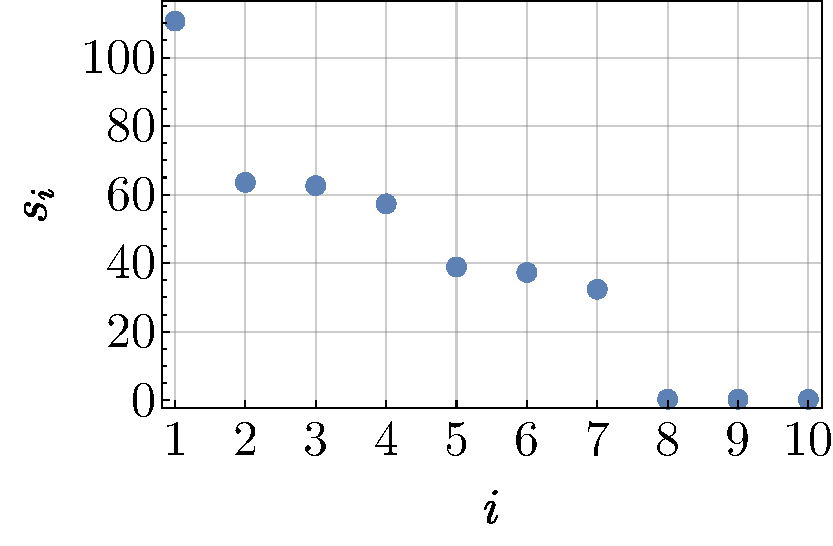
\includegraphics[width=\textwidth]{VVBs-principalValues_sevenNonzero.pdf}
    \end{subfigure}\\
    \centering
    \begin{subfigure}{0.5\textwidth}
        \centering
        \caption{}
        \label{fig:GL:fredkin_diagonal_solutions}
        \hspace{-20pt}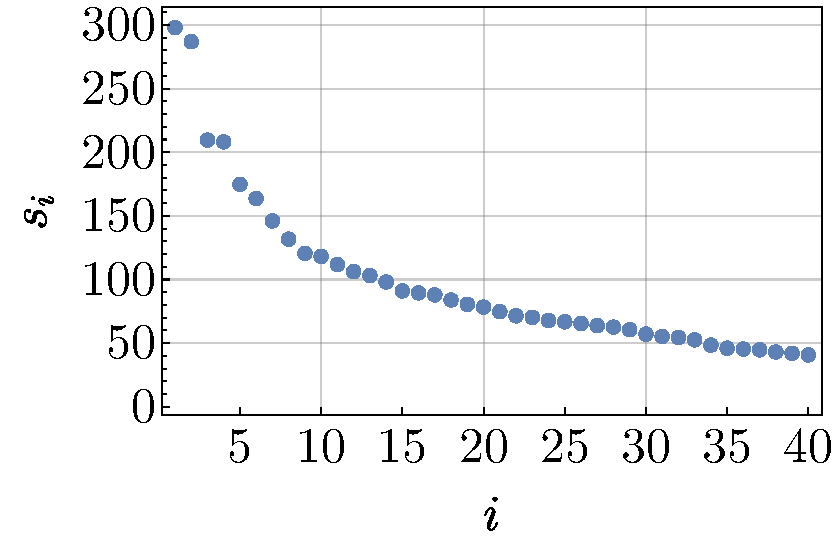
\includegraphics[width=\textwidth]{VVBs-principalValues_fortyNonzero.pdf}
    \end{subfigure}
    \caption{First ten singular values corresponding to the datasets in~\cref{fig:VVBs:principal_components}.
    \textbf{(a)} Singular values computed from the dataset $\calS_1$. Consistently with the results shown in the upper figures in~\cref{fig:VVBs:principal_components}\textbf{a} and the dimensional of the underlying space spanned by $\calS_1$, only the first six singular values are nonzero.
    \textbf{(b)} Singular values computed from the dataset $\calS_2$. There are exactly seven nonzero singular values, consistently with the dimension of the space spanned by $\calS_2$.
    \textbf{(c)} Singular values corresponding to the principal components in~\cref{fig:VVBs:principal_components}\textbf{b} computed from the experimental dataset.
    }
    \label{fig:VVBs:singularValues_sixAndSevenAndForty}
\end{figure}


\tmpHeading{Toy examples of application of PCA to VVBs}
To illustrate the usefulness of these ideas to gain insight into the type of states generated by a given apparatus, we consider two additional example applications of \ac{PCA} to VVBs.
% In all of these cases, \ac{PCA} is applied without any previous knowledge of the type of states that underlie the observed experimental images, and is therefore to be considered a type of \emph{unsupervised learning}.
Consider a set of simulated images corresponding to VVBs of the form
\begin{equation}
c_1\ket{L,m=1}+c_2\ket{R,m=2}
\quad\text{ and }\quad
c_1\ket{L,m=1}+c_2\ket{R,m=4},
\end{equation}
where the coefficients $c_i$ are sampled uniformly at random from the set of $c_{1},c_2\in\mathbb{C}$  such that $|c_1|^2+|c_2|^2=1$.
Applying PCA to this dataset, we find six non-vanishing singular values. The corresponding principal components are given in~\cref{fig:VVBs:principal_components}\textbf{a}, and the associated singular values in~\cref{fig:VVBs:singularValues_sixAndSevenAndForty}\textbf{a}.
This is consistent with the dimension of the subspace  spanned by the states in $\calS_1\equiv\{c_1\ket{L,1}+c_2\ket{R,2}, c_3\ket{L,1}+c_4\ket{R,4}\}$,  as the set of corresponding density matrices is spanned by the six orthogonal matrices
$X^{(1,2)}, X^{(1,4)}, Y^{(1,2)},Y^{(1,4)},Z^{(1,2)}\pm Z^{(1,4)}$, where $X^{(i,j)}=\ketbra{i}{j}+\ketbra{j}{i}$ is the Pauli $X$ matrix acting on the $(i,j)$ subspace, and $Y^{(i,j)}$ and $Z^{(i,j)}$ are similarly defined.
On the other hand, if the dataset under consideration consists of states in the space $\mathcal S_2=\{c_1\ket{L,1}+c_2\ket{R,2}, c_3\ket{L,3}+c_4\ket{R,4}\}$, then \ac{PCA} finds \emph{seven} principal components associated with non-vanishing singular values, as again shown in~\cref{fig:VVBs:principal_components}\textbf{a}. The corresponding singular values are given in~\cref{fig:VVBs:singularValues_sixAndSevenAndForty}\textbf{b}.
This is consistent with the underlying state space being spanned by the seven orthogonal Hermitians:
\begin{equation}
\begin{gathered}
    X^{(1,2)}, X^{(3,4)},
    Y^{(1,2)}, Y^{(3,4)},
    Z^{(1,2)},
    -Z^{(1,2)} + 2 Z^{(1,3)},
    -Z^{(1,2)} - Z^{(1,3)} + 3 Z^{(1,4)}.
\end{gathered}
\end{equation}
These matrices can be derived via direct analysis by finding a set of orthogonal Hermitians generating $\on{span}(\calS_2)$.
This method is thus a quick and easy way to obtain useful information about the dimensionality of generated states, as well as other properties such as specific geometric features, like the sphere emerging from the experimental dataset discussed in the previous paragraph.


\section{Support vector machines}
\label{sec:VVBs:SVMs}


\tmpHeading{What are SVMs?}
\acfp{SVM} are a class of \emph{supervised learning} algorithms whose goal is to classify data into discrete classes. \acp{SVM} work by finding a partition of the feature space such that all the vectors in the same class lie on the same classification sector.
In particular, \emph{linear} \acp{SVM} look for an optimal \emph{linear} separation.
As other supervised learning algorithms, SVMs take as input a training set of labelled data of the form $\{(\bs x_1,\ell_1),...,(\bs x_n,\ell_n)\}$, where $\bs x_i\in\RR^N$ and $\ell_i\in\{-1,1\}$.
A linear separation is characterised by two parameters $\bs w$ and $b$, which identify a hyperplane as the set of $\bs x\in\RR^N$ such that $\bs w\cdot\bs x=b$. We want this hyperplane to be such that, for all training vectors $\bs x_i$, the constraint
\begin{equation}
	\ell_i(\bs w\cdot\bs x_i-b)\ge1
	\label{eq:VVBs:SVMs_basic_condition}
\end{equation}
is satisfied. This would imply that all (and only) the $\bs x_i$ corresponding to $\ell_i=1$ lie on the same side of the hyperplane.
New data is then categorised using the \emph{classifier} $g_{\bs w,b}(\bs x)=2\Theta(\bs w\cdot\bs x-b)-1$, which equals $\pm1$ depending on whether the point $\bs x$ is on one side of the separation or the other.
The constraint in~\cref{eq:VVBs:SVMs_basic_condition} identifies the so-called \emph{hard-margin} SVM, because this is only possible if every single training point is strictly on one or the other side of the separating hyperplane.
An often more practical alternative are the so-called \emph{soft-margin} SVMs, in which this strictness is lifted. Instead, the goal becomes to minimise the average value of
$\max(0, 1- \ell_i (\bs w\cdot\bs x_i- b))$, trying at the same time to keep $\|\bs w\|$ as low as possible. This variation makes the algorithm more robust and able to classify data even in the presence of some noise.

\tmpHeading{SVMs after PCA}
The reduced representations provided by \ac{PCA} can function as starting point to train a classifier with an accuracy comparable with that of the \acp{CNN} used in~\cref{sec:VVBs:CNNs}, while requiring a drastically reduced amount of computational resources.
We use as classifiers linear multiclass \acp{SVM}~\cite{hearst1998support,shawe2000support}, performing training and classification on the reduced representation found via \ac{PCA}. This makes for improved computational times, as well as making the algorithm more robust to experimental noise and imperfections.
As done for the \ac{CNN}, we consider the task of classifying experimentally generated VVBs, categorising images according to their OAM quantum numbers $(m_1,m_2)$.
% What's more, the geometrical picture offered by the reduced representation tells us when we should expect this classification to be accurate: \ac{PCA} effectively retrieves the description of the states in the generalised Bloch representation, therefore the classification will give good results whenever the states are linearly separated in state space.

\tmpHeading{Results}
We use half of the dataset for training, and the other half for testing the resulting accuracy.
We find a \emph{linear} SVM, instead of a more commonly employed SVM with RBF kernel, to give better accuracies: $\sim98\%$ vs the $\sim94\%$ using the RBF kernel.
In~\cref{fig:VVBs:PCAresults}\textbf{d}, we highlight how the average overall accuracy depends on the dimension of the reduced representation: $\sim 25$ dimensions are already sufficient for good accuracies.
A breakdown of the classification performance is reported in~\cref{fig:VVBs:accuracies15classes_SVC}.
In~\cref{fig:VVBs:principal_components}\textbf{b} we report the images corresponding to the first forty principal components derived from this dataset, while in~\cref{fig:VVBs:singularValues_sixAndSevenAndForty}\textbf{c} we give the corresponding singular values.
The average classification accuracy is $\sim 98 \%$. This result confirms that the description provided by \ac{PCA} is sufficient to capture the important features of the generated states, thus allowing for significantly more efficient classification schemes.

\begin{figure}[tb]
	\centering
	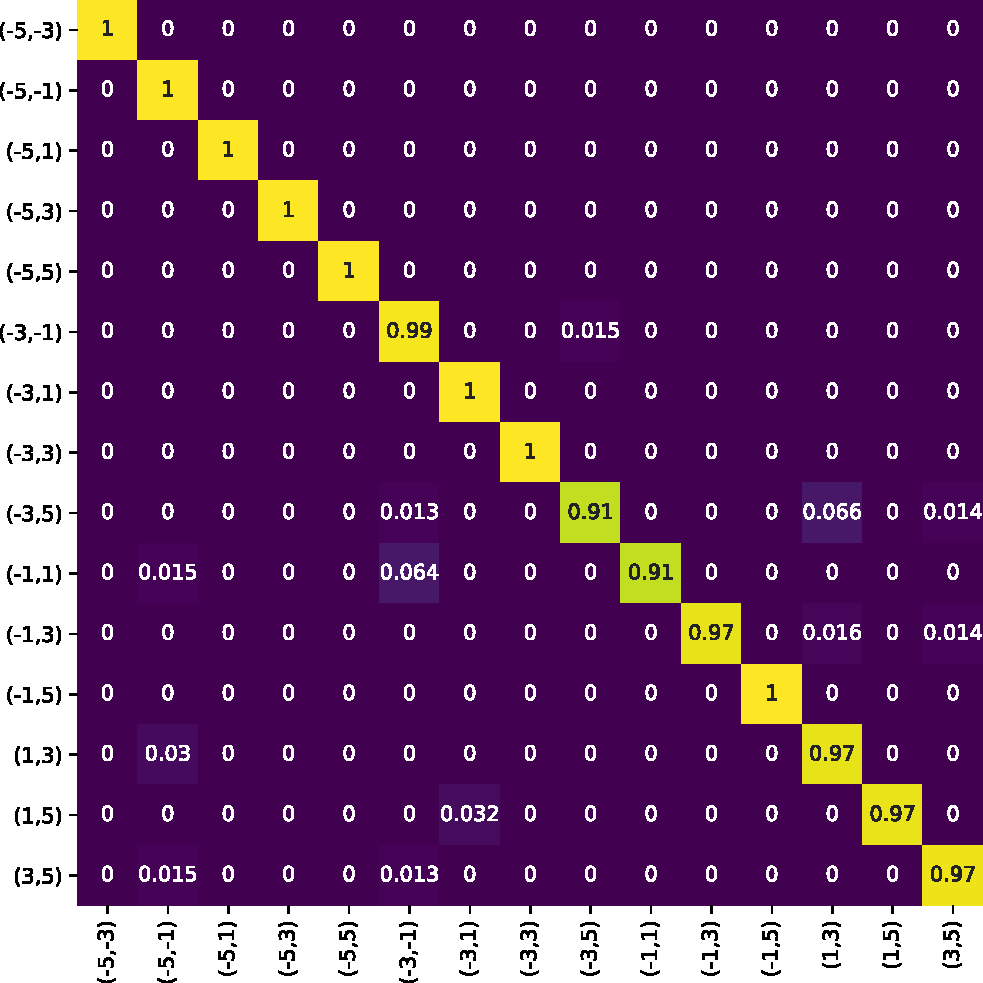
\includegraphics[width=0.7\textwidth]{Figures/VVBs/VVBs-svcAccuracies_15classes_halftrainingdata_40dims_usedInPaper.pdf}
	% 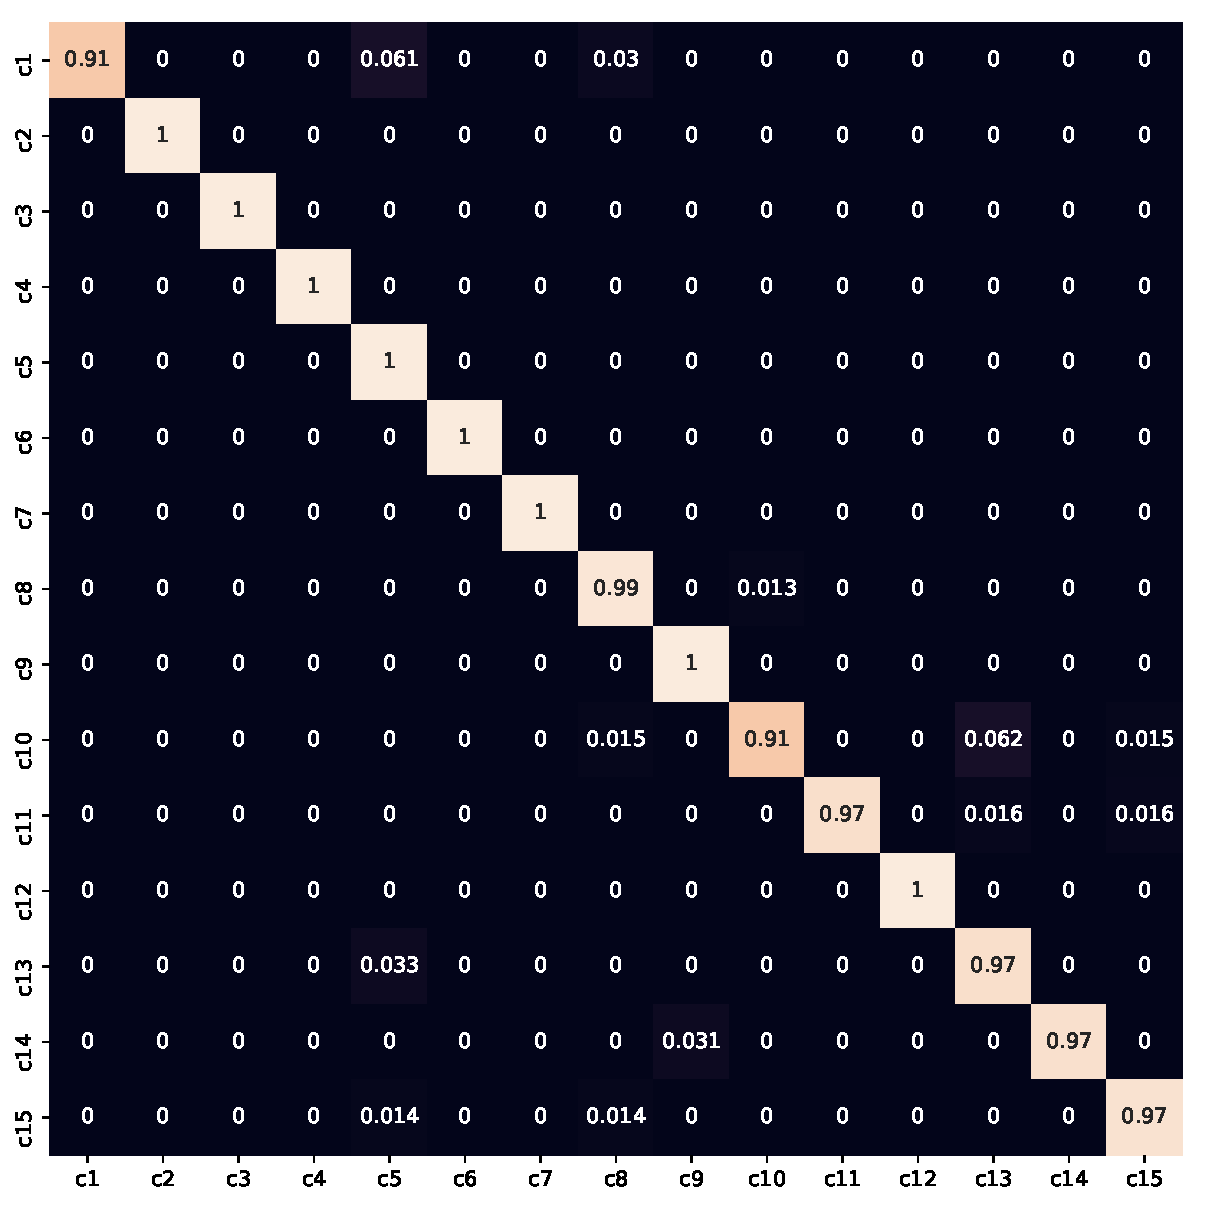
\includegraphics[width=0.9\textwidth]{Figures/VVBs/VVBs-svcAccuracies_15classes_halftrainingdata_40dims_linear.pdf}
	\caption{
		Breakdown of the results obtained using the SVM classifier.
		Each row contains the fraction of states belonging to that class that were classified as belonging to each one of the other classes. The diagonal elements thus give the accuracy of the classifier on each class.
	}
    \label{fig:VVBs:accuracies15classes_SVC}
\end{figure}

\begin{figure}[tb]
	\centering
	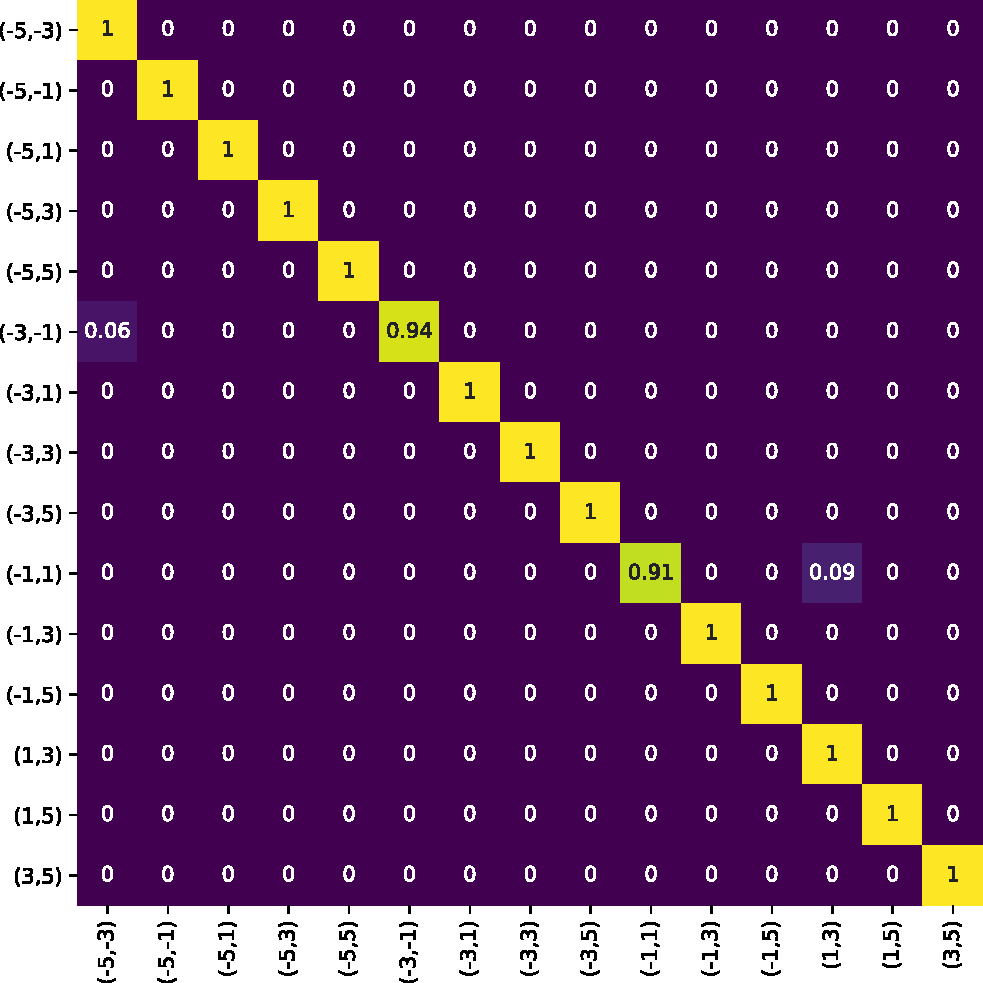
\includegraphics[width=0.7\textwidth]{Figures/VVBs/VVBs-accuracies15classes_CNN2.pdf}
	% 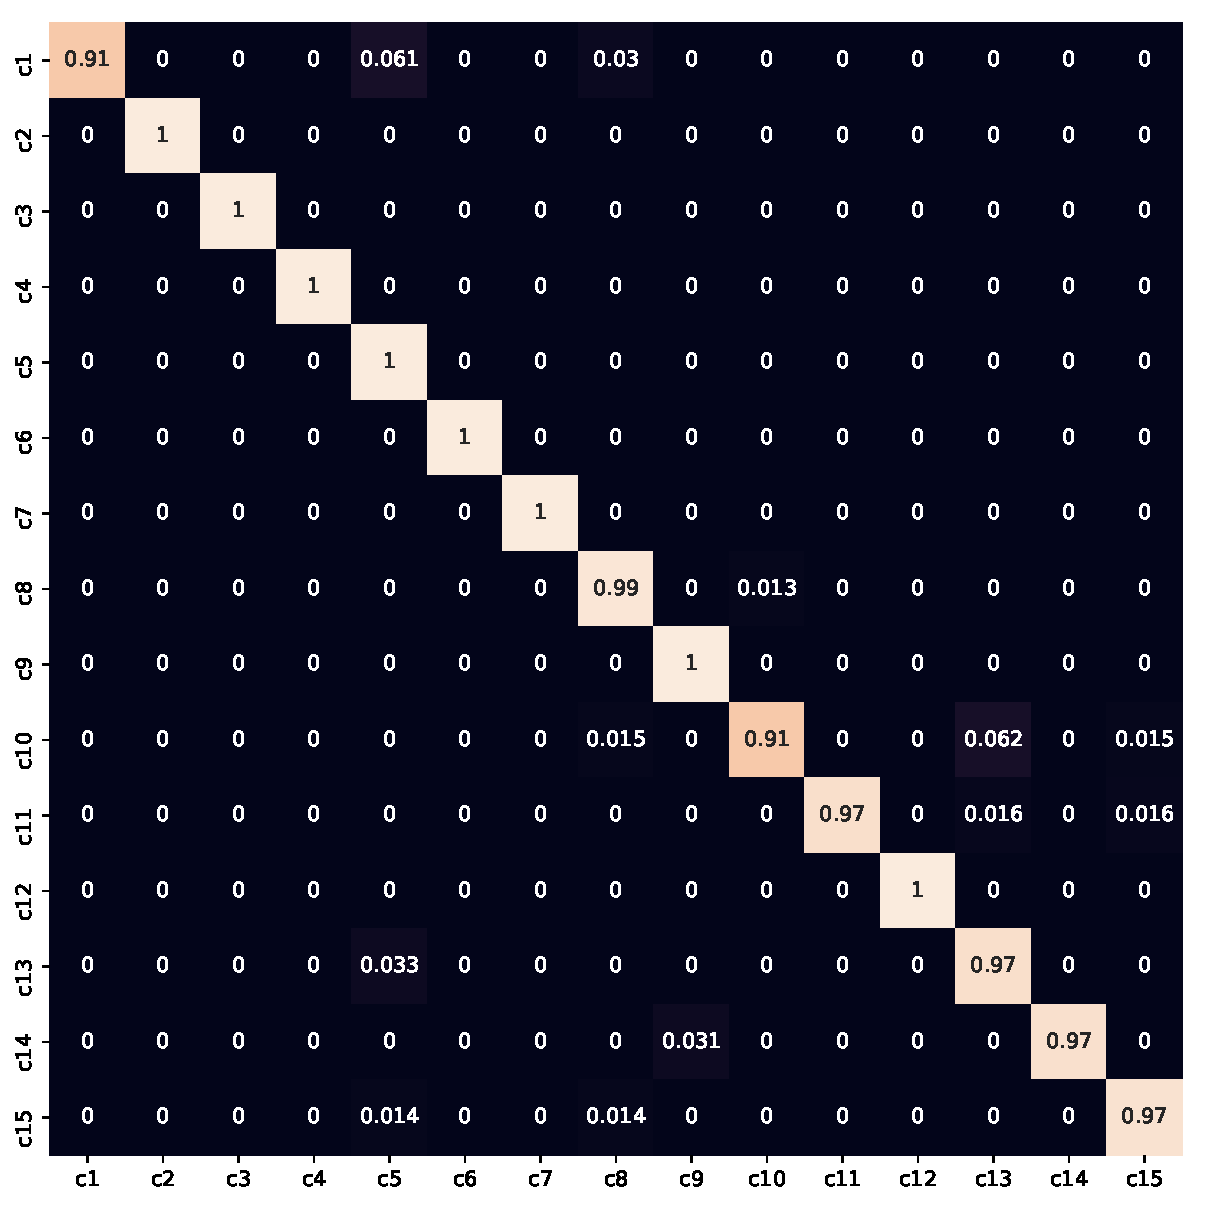
\includegraphics[width=0.9\textwidth]{Figures/VVBs/VVBs-svcAccuracies_15classes_halftrainingdata_40dims_linear.pdf}
	\caption{
		Breakdown of the results obtained using the CNN classifier.
		Each row contains the fraction of states belonging to that class that were classified as belonging to each one of the other classes. The diagonal elements thus give the accuracy of the classifier on each class.
	}
	\label{fig:VVBs:accuracies15classes_CNN}
\end{figure}


\section{Conclusions}
\label{sec:VVBs:conclusions}

We presented a novel approach to classify \acp{VVB} using a combination of supervised and unsupervised learning algorithms. More precisely, we demonstrated how to use standard inference strategies based on CNNs, PCA, and SVMs to probe efficiently high-dimensional photonics \ac{VVB} systems.
In particular, we used dimensionality reduction to probe the underlying geometrical properties of experimentally generated VVBs, without requiring prior knowledge about the physics of the generation apparatus.
% By embedding a variety of \ac{ML} algorithms into our experimental pipeline, the task of characterising structured light is made significantly broader in the methods, ranging from supervised to unsupervised learning, and more flexible in the applications, classification and regression tasks.
%Then, the investigation of different techniques in the ML field has provided a more general framework for the characterization of structured light.  
% While paving the way for further experimental validations, potentially also in non-photonics settings, we believe that numerous tasks of relevance to modern photonics could benefit from introducing similar {\ac{ML}} ideas into their characterisation protocols.
The flexibility of these techniques makes the applicability of our approach extend to a variety of different experimental scenarios.
Moreover, these techniques present a promising add-on to tasks ranging from the design of automatised pipelines to characterise experimental platforms, to the provision of solutions to OAM demultiplexing in the context of classical and quantum communication and, more generally, for the use of structured light in quantum technologies.

